\documentclass[../main]{subfiles}
\usepackage{lastpage,xr,refcount,etoolbox}
%\externaldocument{../Appendices/Appendix1-CodigosBase}
\begin{document}


\chapter{Training a Neural Network is NPC}

{
\hypersetup{linkcolor=black}
\minitoc
\vspace{5mm}
}

In this chapter, after discussing the code implementation and mathematical definitions, we will explain why, even today, training a neural network to function correctly remains an extraordinarily slow and expensive process. 

We will demonstrate that training a neural network is an NPC problem by restricting our case to a network with just 3 nodes. This document will follow the demonstration scheme presented in the article by Avrim L. Blum and Ronald L. Rivest \hyperlink{target}{\textcolor{blue}{[2]}}.
\section{Description of the 3NN Problem}
To begin with, we need to provide an extensive description of the problem we want to prove is NP-complete. To ensure the explanation is both rigorous and easy to understand, we will provide both a formal and an informal definition.

\subsection{Informal definition of the problem}
Given a neural network \(\mathcal{N}\), we informally define the training problem on \(\mathcal{N}\) as follows:
\begin{center}
    \textit{Given a training set, does there exist a set of weights and threshold values such that \(\mathcal{N}\) produces results consistent with the training set?}
\end{center}
\begin{figure}[H]
  \centering
  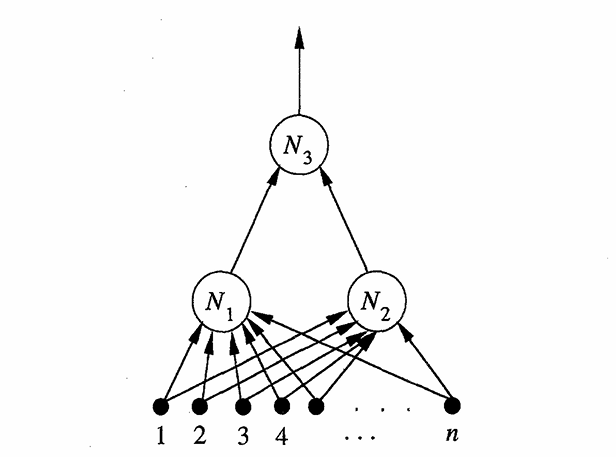
\includegraphics[width=0.5\textwidth]{./figures/modelo}
  \caption{Neural network of 3 nodes}
  \label{fig:red}
\end{figure}

\subsection{Formal Definition of the Problem}

From the image of the neural network \textcolor{blue}{\ref{fig:red}} with 3 nodes and \(n\) input objects, we can derive the function that calculates the value of each node:

\begin{equation*}
    N_i(\Vec{x}) = \begin{cases}
  1 & \text{if } \ a_1x_1 + a_2x_2 + \cdots + a_mx_m > a_0 \\
  0 & \text{otherwise}
\end{cases} \vspace{3mm}
\end{equation*}

\begin{itemize}
    \item[$\bullet$] \(\textbf{N}_i\) is the \(i\)-th node in my neural network \(\mathcal{N}\).
    \item[$\bullet$] \(\Vec{\textbf{x}}\) is the vector of input values for the node \(\textbf{N}_i\).
    \item[$\bullet$] \(\textbf{a}_i\) (\(i \neq 0\)) is the set of weights for the node \(\textbf{N}_i\).
    \item[$\bullet$] \(\textbf{a}_0\) is the threshold for the node \(\textbf{N}_i\).
\end{itemize}
Given this definition of a node in a neural network, we can now derive the formal definition of a neural network \(\mathcal{N}\). A neural network is a tuple \((N, R)\) where \(N\) is the set of nodes in the network and \(R\) is the relation between each node and its set of weights and threshold values:
\begin{equation*}
    \mathcal{N} = (N, R)
\end{equation*}
\begin{equation*}
   N = \{ N_1, N_2, \ldots, N_p \}
\end{equation*}
\begin{equation*}
\begin{aligned}
   R = \{ & (N_1, \{ a_{1,0}, a_{1,1}, a_{1,2}, \ldots, a_{1,n_1} \}), \\
          & (N_2, \{ a_{2,0}, a_{2,1}, a_{2,2}, \ldots, a_{2,n_2} \}), \\
          & \dots, \\
          & (N_p, \{ a_{p,0}, a_{p,1}, a_{p,2}, \ldots, a_{p,n_p} \}) \}
\end{aligned}
\end{equation*}

Given a neural network with \(n\) inputs, a training object would be the set of values that feed into the \(n\) inputs. We can formally define the set of training objects as:

\begin{equation*}
    S = \{ x_1, x_2, \ldots, x_n \}
\end{equation*}
\begin{equation*}
    x_i = (y_i, \text{VR}_i)
\end{equation*}
\begin{equation*}
    y_i = \{ z_{i,1}, z_{i,2}, \ldots, z_{i,k} \}
\end{equation*}
\begin{equation*}
    \text{VR}_i \text{ is the actual value that the network is expected to return when the object } x_i \text{ is input.}
\end{equation*}

We need to define a function \(\mathcal{C}\) that, given a neural network \(\mathcal{N}\) and a set of training objects \(S\), determines whether the neural network is consistent with the set of test objects:

\begin{equation*}
    \mathcal{C}(\langle \mathcal{N}, S \rangle) = \begin{cases}
  \text{true} & \text{if } \mathcal{N} \text{ \textbf{is} consistent with } S \\
  \text{false} & \text{if } \mathcal{N} \text{ \textbf{is not} consistent with } S
  \end{cases}
\end{equation*}

With all these definitions, we can formally define the problem of training a neural network with 3 nodes, which I will refer to from now on as \textbf{3NN}:

\begin{equation*}
    \textbf{3NN} = \{ \langle \mathcal{N}, S \rangle \mid \mathcal{N} = (N, R), |N| = 3, \exists \, \mathcal{N}' = (N, R') \text{ such that } \mathcal{C}(\langle \mathcal{N}', S \rangle) = \text{true} \}
\end{equation*}

\subsection{Simple Valid Example}
Given the complexity of algorithms used in neural networks for learning, let's consider a simple example where each input object has a size of 1. We will have only two input objects:
\begin{center}
    $\textbf{l}_\textbf{1} = (\mathcal{N}, S)$
    
    $S = \{ \, x_1, \, x_2 \, \}, \quad x_1 = (\, y_1, \, \text{VR}_1 \,),  \quad x_2 = (\, y_2, \, \text{VR}_2\, )  $
    
    $y_1 = \{ \, 1 \, \},  \quad y_2 = \{ \, 0 \, \}, \quad \text{VR}_1 = 1, \quad \text{VR}_2 = 0$
    
    $\mathcal{N} = (\, N,\, R \, )$
    
    $N = \{ \, N_1,\, N_2,\, N_3 \, \}$
\end{center}
\begin{equation*}
\begin{aligned}
   R = \{ & (\,N_1, \, \{ \, a_{1,0}, \, a_{1,1} \, \}\,), \\
          & (\,N_2, \, \{ \, a_{2,0}, \, a_{2,1} \, \}\,), \\
          & (\,N_3, \, \{ \, a_{3,0}, \,a_{3,1}, \, a_{3,2} \, \}\,) \, \}
\end{aligned} \vspace{2mm}
\end{equation*}
The question is whether there exists a combination of weights and thresholds for the network such that it is consistent with this small set of test cases. The algorithm that modifies the weight values to fit the test object set is called "backpropagation." This algorithm uses differential calculus and gradient descent to maximize the learning process.

For this small example, we will not use backpropagation to find the ideal set of weights, as it is unnecessary and can be done somewhat intuitively. The goal is simply to demonstrate that such a set of weights exists. Therefore, we could use the following values for the weights and \textbf{\textit{thresholds}}:\vspace{2mm}
\begin{equation*}
\begin{aligned}
   R' = \{ & (\,N_1, \, \{ \, 0, \, 1 \, \}\,), \\
          & (\,N_2, \, \{ \, 0, \, 1 \, \}\,), \\
          & (\,N_3, \, \{ \, 0, \,1, \, 1 \, \}\,) \, \}    
\end{aligned} \vspace{2mm}
\end{equation*}
\begin{equation*}
    N_3 = \text{``output node''}
\end{equation*}
Now, let’s see what the neural network returns with this combination of nodes when we input the test cases. To calculate the value of the output node, we first need to calculate the values of the two internal nodes that receive the input:

\begin{equation*}
    N_1( \, \{ \, y_1 \, \} \,) = \begin{cases}
  \ 1 \ \ & \text{if } \  \ a_{1,1}y_1>a_{1,0} \\
  \ 0 & \text{otherwise }  
\end{cases}  \rightarrow \ N_1(\, \{ \, 1 \, \}\,) = 1\vspace{3mm}
\end{equation*}
\begin{equation*}
    N_2(\, \{ \, y_1 \, \}\,) = \begin{cases}
  \ 1 \ \ & \text{if } \  \ a_{2,1}y_1>a_{2,0} \\
  \ 0 & \text{otherwise }  
\end{cases}  \rightarrow \ N_2(\, \{ \, 1 \, \}\,) = 1\vspace{3mm}
\end{equation*}
\begin{equation*}
    N_3(\, \{ \, N_1(1), \, N_2(1)\, \} \,) = N_3(\, \{ \, 1, \, 1\, \} \,) = \begin{cases}
  \ 1 \ \ & \text{if } \  \ a_{3,1}(1)+a_{3,2}(1)  >a_{3,0} \\
  \ 0 & \text{otherwise }  
\end{cases}  \rightarrow \ N_3(\, \{ \, 1, \, 1\, \} \,) = 1\vspace{3mm}
\end{equation*}
\begin{equation*}
    \mathcal{N}(y_1) = 1 \land \text{VR}_1 = 1
\end{equation*}
The neural network with the selected weights has been able to accurately predict the actual value of the first object. Now let’s see what happens with the second object:
\begin{equation*}
    N_1( \, \{ \, y_2 \, \} \,) = \begin{cases}
  \ 1 \ \ & \text{if } \  \ a_{1,1}y_2>a_{1,0} \\
  \ 0 & \text{otherwise }  
\end{cases}  \rightarrow \ N_1(\, \{ \, 1 \, \}\,) = 0\vspace{3mm}
\end{equation*}
\begin{equation*}
    N_2(\, \{ \, y_2 \, \}\,) = \begin{cases}
  \ 1 \ \ & \text{if } \  \ a_{2,1}y_2>a_{2,0} \\
  \ 0 & \text{otherwise }  
\end{cases}  \rightarrow \ N_2(\, \{ \, 1 \, \}\,) = 0\vspace{3mm}
\end{equation*}
\begin{equation*}
    N_3(\, \{ \, N_1(1), \, N_2(1)\, \} \,) = N_3(\, \{ \, 1, \, 1\, \} \,) = \begin{cases}
  \ 1 \ \ & \text{if } \  \ a_{3,1}(1)+a_{3,2}(1)  >a_{3,0} \\
  \ 0 & \text{otherwise }  
\end{cases}  \rightarrow \ N_3(\, \{ \, 1, \, 1\, \} \,) = 0\vspace{3mm}
\end{equation*}
\begin{equation*}
    \mathcal{N}(y_2) = 0 \land \text{VR}_2 = 0
\end{equation*}
The neural network has also been able to accurately predict the actual value of the second object. This demonstrates that this neural network $\mathcal{N}$ with this assignment of weights and thresholds has been able to produce consistent results on the training set $\mathcal{S}$, therefore:
\begin{equation*}
   \textbf{l}_\textbf{1} \in \textbf{3NN}
\end{equation*}

\subsection{Simple Invalid Example}
As such, given a neural network $\mathcal{N}$ and a training set, with a sufficient number of iterations it usually manages to adapt successfully to the test cases. However, since we are working with a neural network with only 3 nodes, if we create a training set that is quite large and make each value very similar to each other but with different images, it is very likely that the neural network will not be able to adapt to the test cases. For example:
\begin{equation*}
    \textbf{l}_\textbf{2} = (\mathcal{N}', S')
\end{equation*}
\begin{equation*}
  S' = \{ \, \{ \, 1,\,1 \,\}, \, \{ \, 0'99,\,0 \,\}, \, \{ \, 0'98,\,1 \,\}, \, \{ \, 0'97,\,0 \,\}, \, \{ \, 0'96,\,1 \,\}, \, \{ \, 0'95,\,0 \,\} \}
\end{equation*}
\begin{equation*}
    \mathcal{N}' = (\, N',\, R' \, )
\end{equation*}
\begin{equation*}
   N' = \{ \, N_1,\, N_2,\, N_3 \, \}
\end{equation*}
\begin{equation*}
\begin{aligned}
   R' = \{ & (\,N_1, \, \{ \, a_{1,0}, \, a_{1,1} \, \}\,), \\
          & (\,N_2, \, \{ \, a_{2,0}, \, a_{2,1} \, \}\,), \\
          & (\,N_3, \, \{ \, a_{3,0}, \,a_{3,1}, \, a_{3,2} \, \}\,) \, \}
\end{aligned} \vspace{2mm}
\end{equation*}
It is almost impossible for a neural network with only 3 nodes to accurately distinguish the values given the training set $S'$ due to their similarity. Because of this:
\begin{equation*}
   \textbf{l}_\textbf{2} \notin \textbf{3NN}
\end{equation*}
\subsection{Application Areas}
Artificial neural network models have a multitude of applications and uses in our daily lives. Here are just a few of the many areas where neural networks are transforming the way we interact with technology and tackle complex problems:
\begin{itemize}
\item[\textbullet] \textbf{Voice Recognition}: Used in virtual assistant systems like Siri, Alexa, or Google Assistant to convert speech into text and perform actions.
\item[\textbullet] \textbf{Image Recognition}: Employed in facial recognition applications, object classification in photographs, and security systems such as video surveillance.
\item[\textbullet] \textbf{Natural Language Processing (NLP)}: Applied in machine translation, sentiment analysis on social media, automatic text generation, and chatbots.
\item[\textbullet] \textbf{Autonomous Driving}: In autonomous vehicles to detect pedestrians, vehicles, and traffic signs, and make real-time decisions.
\item[\textbullet] \textbf{Recommendation Systems}: Used by streaming platforms like Netflix and Spotify to recommend movies, music, or products to users.
\item[\textbullet] \textbf{Finance}: In credit risk analysis, fraud detection, and market price prediction.
\item[\textbullet] \textbf{Medicine}: In medical diagnosis, analysis of medical images such as X-rays and MRIs, and drug development.
\end{itemize}
\section{3NN $\in$ NP}
In the process of proving the NP-completeness of \textbf{3NN}, the first step is to demonstrate that it belongs to the class NP. To achieve this, there are two approaches. For this report, we will prove that \textbf{3NN} $\in$ \textbf{NP} by showing that it has a verifier that operates in polynomial time.

\subsection{Verifier for 3NN}
In the verifier-based proof, the goal is to show that an algorithm $\mathcal{V}$ that operates in polynomial time is capable of verifying whether a certificate or proof $\mathcal{P}$ belongs to the language.
\begin{equation*}
    \textbf{3NN} = \{\, \langle \mathcal{N}, \, S \rangle \ \ | \ \  \mathcal{N} = (\, N, \, R \, ), \ \, | \, N \, | = 3, \ \, \exists \, \mathcal{N}' = (\, N, \, R' \, ) \, : \, \mathcal{C}(\, \langle \mathcal{N}', \, S \rangle \,) = \text{true} \, \}
\end{equation*}
\begin{center}
    $\mathcal{N}'$ \text{ is the certificate } $\mathcal{P}$
\end{center}
\subsubsection{Specification of the Algorithm $\mathcal{V}$}
$\mathcal{V}$ takes as input $\langle\langle \mathcal{N}, \, S \rangle, \, \mathcal{N}' \rangle$
\begin{enumerate}
\item[\textbf{1.}] Check if $\mathcal{N}'$ is consistent with the training set $S$. Specifically, verify that $\mathcal{C}(\langle \mathcal{N}', \, S \rangle) = \text{true}$.
\item[\textbf{2.}] Check if $\mathcal{N}$ contains all the nodes $N_i$ in $\mathcal{N}'$.
\item[\textbf{3.}] If steps 1 and 2 are satisfied, accept. Otherwise, reject.
\end{enumerate}

\subsubsection{Complexity of the Algorithm $\mathcal{V}$}
The complexity of the algorithm $\mathcal{V}$ can be computed by summing the complexities of steps 1 and 2 separately (since step 3 is a constant-time action). Step 2 also has constant complexity because we are dealing with neural networks of 3 nodes. This means that the complexity of the algorithm is determined by step 1. \\ \\
The input to this problem is the training set. Each training object has a size $k$ (number of ``inputs'' to the neural network), so the size of the input for $n$ training objects follows the expression:
\begin{equation*}
    \text{size} = n \times k
\end{equation*}
For each training object, each of the two internal nodes of our network must perform $k$ operations. Finally, the node that computes the result from the two internal nodes evaluating object $i$ performs two additional operations. Thus, the number of operations to evaluate the neural network with object $i$ follows the expression: 
\begin{equation*}
    \text{image}(n_i) = 2k + 2
\end{equation*}
This means that the number of operations $t(n)$ required for the algorithm to verify step 1 is:
\begin{equation*}
    t(n,\,k) = n(2k + 2) = 2kn + 2n
\end{equation*}
\begin{equation*}
    t(n,\,k) \in O(n \cdot k)
\end{equation*}
This demonstrates that the algorithm $\mathcal{V}$ can verify in \textbf{poly-time} whether the certificate $\mathcal{P}$ belongs to \textbf{3NN}. Therefore, it guarantees that:
\begin{equation*}
    \textbf{3NN} \in \textbf{NP}
\end{equation*}
\section{3NN $\in$ NPC}
To prove that a problem is \textbf{NP-complete}, we generally follow the same reasoning framework. We either demonstrate that any problem in \textbf{NP} can be reduced to it, or we reduce a problem that has already been proven to be \textbf{NP-complete} to it: \vspace{1mm}
\begin{center}
    $B \in \textbf{NPC} \Longleftrightarrow [(\, \forall A \in \textbf{NP}\ :\ A \leq_p B\, ) \land (\,B \in \textbf{NP}\, )]$
    $B \in \textbf{NPC} \Longleftrightarrow
[(A \in \textbf{NPC}) \land (B \in \textbf{NP}) \land (A \leq_p B)]$
\end{center} 
For this demonstration, we will choose the first approach. We will introduce a problem that has already been proven to be \textbf{NP-complete} and show that a polynomial reduction can be performed to it.
\subsection{The SS Problem}
The problem that is \textbf{NP-complete} and that we will use for the reduction is the \textbf{Set-Splitting} problem, which from now on I will refer to as \textbf{SS}. It was proven \textbf{NP-complete} by `László Lovász' \hyperlink{target:zona}{\textcolor{blue}{[4]}}.

\subsubsection{Informal Definition of the Problem}
\begin{center}
    \textit{Given a finite set \textbf{S} and a collection \textbf{C} of subsets $\textbf{c}_\textbf{i}$ of \textbf{S}, do there exist two disjoint sets $\textbf{S}_\textbf{1}$, $\textbf{S}_\textbf{2}$ such that $\textbf{S}_\textbf{1} \cup \textbf{S}_\textbf{2} = \textbf{S}$ and for every $\textbf{c}_\textbf{i} \not\subset \textbf{S}_\textbf{1}$ and $\textbf{c}_\textbf{i} \not\subset \textbf{S}_\textbf{2}$?}
\end{center}

\subsubsection{Formal Definition of the Problem}
\begin{equation*}
    \textbf{SS} = \{\, \langle \textbf{S}, \, \textbf{C} \rangle \ \ | \ \ \exists \, \textbf{S}_\textbf{1},\, \textbf{S}_\textbf{2} \, : \, (\,\textbf{S}_\textbf{1} \cup \textbf{S}_\textbf{2} = \textbf{S}\,) \land (\,\forall \textbf{c}_\textbf{i} \in \textbf{C} \,: \, \textbf{c}_\textbf{i} \not\subset \textbf{S}_\textbf{1} \land \textbf{c}_\textbf{i} \not\subset \textbf{S}_\textbf{2}\,)\, \}
\end{equation*}
\subsubsection{Valid Simple Example}
Let's construct an instance of the \textbf{SS} problem that \textbf{is} valid. To do this, I will construct an arbitrary set \( S \) and an arbitrary collection of subsets (each contained in \( S \)):
\begin{equation*}
    \textbf{l}_\textbf{1} = ( S, \, C )
\end{equation*}
\begin{equation*}
    S = \{ \, 1, \, 2, \, 3, \, 4 \, \} \quad C = \{ \, c_1, \, c_2, \, c_3 \, \}
\end{equation*}
\begin{equation*}
    c_1 = \{ \, 1, \, 2 \, \} \quad c_2 = \{\, 2, \, 3\, \} \quad c_3 = \{\, 3, \, 4\, \} 
\end{equation*}
Now, let’s construct two sets \( S_1 \) and \( S_2 \) such that they satisfy the conditions to belong to the language \textbf{SS}:
\begin{equation*}
    S_1 = \{ \, 1, \, 3 \, \} \quad S_2 = \{\, 2, \, 4 \, \}
\end{equation*}
\begin{equation*}
    (S_1 \cup S_2 = S) \land (c_1 \not\subset S_1) \land (c_1 \not\subset S_2) \land (c_2 \not\subset S_1) \land (c_2 \not\subset S_2) \land (c_3 \not\subset S_1) \land (c_3 \not\subset S_2)
\end{equation*}
\begin{equation*}
    \textbf{l}_\textbf{1} \in \textbf{SS}
\end{equation*}

\subsubsection{Invalid Simple Example}
Let's construct an instance of the \textbf{SS} problem that \textbf{is not} valid. To do this, I will construct an arbitrary set \( S' \) and an arbitrary collection of subsets (each contained in \( S' \)):
\begin{equation*}
    \textbf{l}_\textbf{2} = ( S', \, C' )
\end{equation*}
\begin{equation*}
    S' = \{ \, 1, \, 2, \, 3 \, \} \quad C' = \{ \, c_1', \, c_2', \, c_3' \, \}
\end{equation*}
\begin{equation*}
    c_1' = \{ \, 1, \, 2 \, \} \quad c_2' = \{\, 2, \, 3\, \} \quad c_3' = \{\, 1, \, 3\, \} 
\end{equation*}

Now, let’s show that there is no pair of sets whose union is \( S' \) that satisfies the remaining restrictions:

\begin{center}
$S_1 = \{1, 2, 3\}, \ S_2 = \emptyset \rightarrow c_1' \subset S_1 \rightarrow \textbf{l}_\textbf{2} \notin \textbf{SS}$
\end{center}
\begin{center}
$S_1 = \emptyset, \ S_2 = \{1, 2, 3\} \rightarrow c_1' \subset S_2 \rightarrow \textbf{l}_\textbf{2} \notin \textbf{SS}$
\end{center}
\begin{center}
$S_1 = \{1, 2\}, \ S_2 = \{3\} \rightarrow c_1' \subset S_1 \rightarrow \textbf{l}_\textbf{2} \notin \textbf{SS}$
\end{center}
\begin{center}
$S_1 = \{3\}, \ S_2 = \{1, 2\} \rightarrow c_1' \subset S_2 \rightarrow \textbf{l}_\textbf{2} \notin \textbf{SS}$
\end{center}
\begin{center}
$S_1 = \{2, 3\}, \ S_2 = \{1\} \rightarrow c_2' \subset S_1 \rightarrow \textbf{l}_\textbf{2} \notin \textbf{SS}$
\end{center}
\begin{center}
$S_1 = \{1\}, \ S_2 = \{2, 3\} \rightarrow c_2' \subset S_2 \rightarrow \textbf{l}_\textbf{2} \notin \textbf{SS}$
\end{center}
\begin{center}
$S_1 = \{1, 3\}, \ S_2 = \{2\} \rightarrow c_3' \subset S_1 \rightarrow \textbf{l}_\textbf{2} \notin \textbf{SS}$
\end{center}
\begin{center}
$S_1 = \{2\}, \ S_2 = \{1, 3\} \rightarrow c_3' \subset S_2 \rightarrow \textbf{l}_\textbf{2} \notin \textbf{SS}$
\end{center}

For each and every possible pair of sets \( S_1 \) and \( S_2 \), the language membership check for the problem resulted in non-membership. This implies that:
\begin{equation*}
    \textbf{l}_\textbf{2} \notin \textbf{SS}
\end{equation*}
\subsubsection{Fields of Application}
The \textbf{SS} problem has applications in various branches of science. Here are some examples:

\begin{itemize}
    \item[\textbullet] \textbf{Graph Theory}: In graph theory, \textbf{SS} can be used to find partitions in a graph where each subset forms a connected component.
    \item[\textbullet] \textbf{Combinatorial Optimization}: In optimization problems, it is often required to divide a set into subsets in a way that satisfies certain constraints, such as minimizing the number of subsets or maximizing some objective function.
    \item[\textbullet] \textbf{Network Design}: In network design, it can be useful to partition a set of nodes into disjoint subsets representing different components or segments of the network.
    \item[\textbullet] \textbf{Algorithm Analysis}: \textbf{SS} can be useful in algorithm analysis to demonstrate the complexity of certain problems or to design efficient algorithms to solve them.
    \item[\textbullet] \textbf{Scheduling}: In scheduling, \textbf{SS} can be used to allocate resources to different time periods in such a way that no conflicts occur between them.
    \item[\textbullet] \textbf{Database Processing}: In database processing, \textbf{SS} can be useful for partitioning large datasets into smaller subsets for analysis and processing.
    \item[\textbullet] \textbf{Cryptography}: In cryptography, \textbf{SS} can be applied to divide secrets into parts that must be combined to recover the original information.
\end{itemize}

\subsection{Reduction from SS to 3NN}
As we have discussed before, we will demonstrate that \textbf{3NN} is an \textbf{NP-complete} problem by constructing a polynomial-time reduction to \textbf{SS}:
\begin{equation*}
\text{3NN} \in \textbf{NPC} \Longleftrightarrow
[(\text{SS} \in \textbf{NPC}) \land (\text{3NN} \in \textbf{NP}) \land (\text{SS} \leq_p \text{3NN})] 
\end{equation*}
\begin{equation*}
\text{SS} \leq_p \text{3NN} 
\end{equation*}
\begin{equation*}
\exists f : \forall w \in \text{SS} \Longleftrightarrow f(w) \in \text{3NN}
\end{equation*}
\begin{equation*}
\textbf{f operates in poly-time}
\end{equation*}

\subsubsection{3NN from the Geometric Point of View}
Before proceeding to the proof of the aforementioned bi-implication, it will be very useful to view the \textbf{3NN} problem from a geometric perspective. In this way, a training object can be understood as a point in the \textbf{boolean} n-dimensional space:
\begin{equation*}
    x_i = \{\,\{ \, 0,\, 1 \, \}^n, \, \,\{\, +' \ | \ -'\,\} \,\}
\end{equation*}
In this manner, the value of each of the points can be +' or -' depending on whether they are an object with value 1 or -1. Due to the presence of the \textbf{Threshold} function in each of the two internal nodes $\textbf{N}_\textbf{1}$ and $\textbf{N}_\textbf{2}$, these can be interpreted as planes in the defined \textbf{boolean} space. $\textbf{N}_\textbf{1}$ and $\textbf{N}_\textbf{2}$ divide the space into 4 quadrants due to the 4 possible pairs of values resulting from their calculation:
\begin{center} $(\textbf{N}_\textbf{1}, \textbf{N}_\textbf{2}
) = (+1, +1)$ \end{center}
\begin{center} $(\textbf{N}_\textbf{1}, \textbf{N}_\textbf{2}
) = (-1, -1)$ \end{center}
\begin{center} $(\textbf{N}_\textbf{1}, \textbf{N}_\textbf{2}
) = (+1, -1)$ \end{center}
\begin{center} $(\textbf{N}_\textbf{1}, \textbf{N}_\textbf{2}
) = (-1, +1)$ \end{center}
If the planes are parallel, it means that 1 or 2 of the quadrants do not exist (they are overlapping). Since the outer node $\textbf{N}_\textbf{3}$ receives the values resulting from the calculation of $\textbf{N}_\textbf{1}$ and $\textbf{N}_\textbf{2}$, it is only capable of distinguishing between points in different quadrants. That is, if it receives a pair of values indicating that the points are in the same quadrant, such as (+1, +1), it should return '+'. 
With all this said, we can assume that the \textbf{3NN} problem is equivalent to the one defined below which we will call \textbf{CEB}:\\\\
Given a collection of points belonging to $\{\, 0, \, 1 \, \}^n$ and that can have as an image +' or -', does any of the following options exist?\vspace{3mm}

\begin{center}
\textit{A single plane that separates the points with '+' label from those with '-' label?}

or

\textit{Two planes that partition the points such that either one quadrant contains all the points with '+' label or one quadrant contains all the points with '-' label?} \vspace{3mm}
\end{center}

In the context of proving the bidirectional implication, it will be much simpler to work with a restricted version of \textbf{CEB}. We will call it the problem of the quadrant of positive \textbf{boolean} examples or simply \textbf{CEBP}. It will be defined as follows:
\begin{center}
\textit{Given O(n) points that belong to ${, 0, , 1 , }^n$ and can have a '+' or '-' label, do there exist two planes that partition the points such that one quadrant contains all the points with a '+' label and none with a '-' label?}
\end{center}
\begin{figure}[H]
\centering
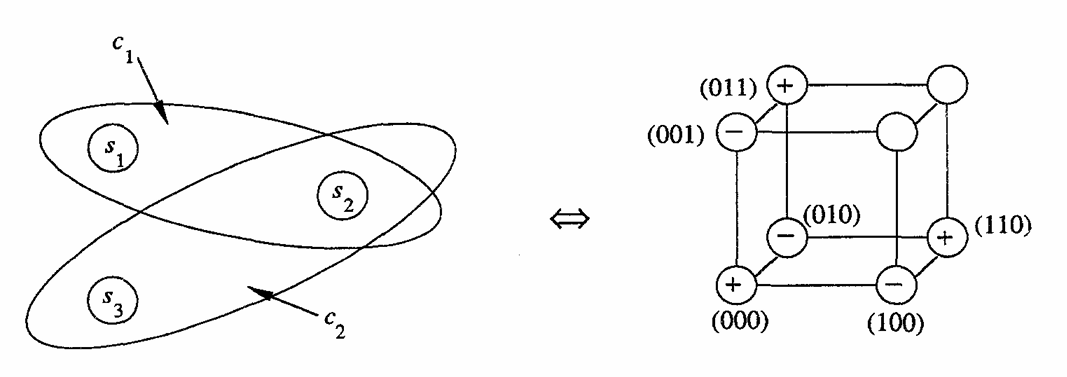
\includegraphics[width=1\textwidth]{./figures/transformacion}
\caption{Conceptual transformation}
\label{fig:concepto}
\end{figure}
Once we have demonstrated that this is \textbf{NP-complete}, we will extend the proof to the full problem by adding examples that do not allow the other possibilities at the output node.

\subsubsection{First Direction of the Implication}
The idea in the first direction of the implication is that given an instance of \textbf{SS}, we can convert it into an instance of \textbf{CEBP} (which will later be extended to \textbf{CEB}) such that the constructed instance has a solution if and only if the instance of \textbf{SS} had a solution:
\begin{equation*}
\exists f : \forall w \in \text{SS} \Longrightarrow f(w) \in \text{CEBP}
\end{equation*}
That is, given an arbitrary instance of the ``Set-Splitting'' problem such as:
\begin{equation*}
    S = \{ \, s_1, \, s_2, \, ..., \, s_i \, \} \quad | \, S \, | = n
\end{equation*}
\begin{equation*}
    C = \{ \, c_1, \, c_2, \, ..., \, c_j \, \} \ : \ c_k \subset S
\end{equation*}
We will create the following points in the n-dimensional \textbf{boolean} space as follows:
\begin{itemize}
    \item[\textbullet] The origin point will be $(\,0^n, \, `+'\,)$
    \item[\textbullet] For each value $s_i$, a point with '-' label will be created with all 0s and a 1 in position i $\rightarrow (\,\stackrel{1}{0}\stackrel{2}{0}...\stackrel{i}{1}...\stackrel{n-1}{0}\stackrel{n}{0}, \, `-'\,) $
    \item[\textbullet] For each $c_k$, a point with '+' label will be created with 1s in the positions i where $s_i \in c_k$ and 0s in the remaining positions.
\end{itemize}

Now we demonstrate that the constructed instance of the \textbf{CEBP} problem has a solution if the given instance of the \textbf{SS} problem had one. For this, given $S_1$, $S_2$ (solution of the \textbf{SS} instance):
\begin{equation*}
    P_1 \equiv a_1x_1 + ... + a_nx_n = - \frac{1}{2} \quad \quad P_1 \equiv b_1x_1 + ... + b_nx_n = - \frac{1}{2}
\end{equation*}
\begin{equation*}
    a_i = \begin{cases}
  \ -1 \ \ & \text{if } \  \ s_i \in S_1 \\
  \ \ \ n & \text{if }  \ \ s_i \notin S_1
\end{cases}
\quad \quad b_i = \begin{cases}
  \ -1 \ \ & \text{if } \  \ s_i \in S_2 \\
  \ \ \ n & \text{if }  \ \ s_i \notin S_2
\end{cases}
\end{equation*}
\begin{center} $\Vec{a} = ( a_1, \, a_2, \, ..., \, a_n )$ \end{center}
\begin{center} $\Vec{b} = ( b_1, \, b_2, \, ..., \, b_n )$ \end{center}
\begin{center} $\Vec{x} = ( x_1, \, x_2, \, ..., \, x_n )$ \end{center}

Due to the way they have been constructed, for each point $\Vec{x}$ with a '+' label, it is guaranteed that $\Vec{x}*\Vec{a}  > -\frac{1}{2}$. Thus, both the quadrant $\Vec{x}*\Vec{a}> -\frac{1}{2}$ and the quadrant $\Vec{x}*\Vec{b}> -\frac{1}{2}$ contain all the points with a '+' label and none with a '-' label. $P_3$ handles distinguishing whether the planes $P_1$ and $P_2$ are parallel (returning '+') or not (returning '-') to produce the final result as seen in {\textcolor{blue}{\ref{fig:concepto}}}.

\subsubsection{Second Sense of Implication}
The idea in the second sense of implication is that given an instance of \textbf{CEBP}, we should be able to convert it to an instance of \textbf{SS} such that the constructed instance has a solution if and only if the \textbf{CEBP} instance had a solution:
\begin{equation*}
\forall f(w) \in \text{CEBP} \Longrightarrow w \in \text{SS}
\end{equation*}
This is equivalent to proving that given an instance that does not belong to \textbf{SS}, the transformation returns an instance that does not belong to \textbf{CEBP}:
\begin{equation*}
\forall w \notin \text{SS} \Longrightarrow f(w) \notin \text{CEBP}
\end{equation*}
As such, we have already constructed and demonstrated how the "gadget" works. However, I will emphasize that if the given instance of the \textbf{SS} problem has no solution, when constructing the list of points, our planes will not be able to separate all points with image `+' from those with image `-'. This is because the positions will overlap, and when we calculate the result by summing the weights, we will obtain values that do not satisfy the established properties.

\subsubsection{Extension of ``CEBP'' to ``CEB''}
It is necessary to extend the transformation a bit because with \textbf{CEBP}, we are not making an equivalence with \textbf{3NN} because we are restricting the exterior node to perform an ``AND'' operation with the results of the two interior nodes. However:
\begin{equation*}
    \textbf{3NN} \equiv \textbf{CEB}
\end{equation*}
\begin{equation*}
(\exists f : \forall w \in \text{SS} \Longleftrightarrow f(w) \in \text{CEB}) \equiv (\exists f : \forall w \in \text{SS} \Longleftrightarrow f(w) \in \text{3NN})
\end{equation*}
Proving the bi-implication for \textbf{CEB} involves accepting different modes of operation for the exterior node (not just an ``AND''). To achieve this, given an instance of \textbf{SS}, we follow the same steps as in \textbf{CEBP} but add 3 new dimensions $x_{n+1}$, $x_{n+2}$, and $x_{n+3}$ and add the following points to the list of points created:
\begin{center}
    (\,0\,... \, 0101,\, `+'\,)\,, \ (\,0\,... \, 0011,\, `+'\,)\,, \ (\,0\,... \, 0100,\, `-'\,)\,, \ (\,0\,... \, 0010,\, `-'\,)\,, \
    
    (\,0\,... \, 0001,\, `-'\,)\,, \ (\,0\,... \, 0111,\, `-'\,)
\end{center}
The points with `+' in these 3 new dimensions can be separated from those with `-' by appropriately calibrating the weights of $P_1$ and $P_2$ corresponding to these 3 new dimensions. In this way, the equations of the original planes can be expanded to the following:

\begin{center}
    $P_1 \equiv a_1x_1 + ... + a_nx_n + x_{n+1} + x_{n+2} - x_{n+3} = - \frac{1}{2}$
    
    $P_1 \equiv b_1x_1 + ... + b_nx_n-x_{n+1}-x_{n+2}+x_{n+3} = - \frac{1}{2}$
\end{center}
\begin{equation*}
    a_i = \begin{cases}
  \ -1 \ \ & \text{if } \  \ s_i \in S_1 \\
  \ \ \ n & \text{if }  \ \ s_i \notin S_1
\end{cases}
\quad \quad b_i = \begin{cases}
  \ -1 \ \ & \text{if } \  \ s_i \in S_2 \\
  \ \ \ n & \text{if }  \ \ s_i \notin S_2
\end{cases}
\end{equation*}
The rest of the points remain as they were. Only 3 zeros are added to each point to account for the 3 new dimensions included. With this change in the plane equations, $P_1$ can separate the point (0...0001, `-') from those with `+', while $P_2$ can separate the other 3 new points with `-' from those with `+'.\\\\
With this solution, we do meet the problem constraints of \textbf{CEB} since neither of the two planes alone is capable of separating the points with `+' from the new points with `-'. There is also no way for the two planes to confine all the points with `-' into the same quadrant. Because of this, any solution to the \textbf{3NN} problem must have all the points with `+' in the same quadrant and also provide a solution to the \textbf{SS} problem.

\subsubsection{Complexity of the Transformation}
After explaining the process of creating the transformation function, it is quite evident that it operates in polynomial time, but it is still necessary to calculate its complexity to complete the proof of \textbf{NP-completeness}. When the transformation is performed, it creates an ``origin'' point; as many points with `-' as there are values in the set \textbf{S}; and as many points with `+' as there are subsets of \textbf{S} in \textbf{C}. Six extra points are added at the end, representing the 3 new dimensions of the extended solution. In the input of the \textbf{SS} problem:
\begin{center}
    \textbf{t} = $| \ S \ |$

    \textbf{k} = $| \ C \ |$
\end{center}
Each point consists of (t+3) 0s and 1s. The size occupied by all the points created by our transformation can be expressed in terms of the \textbf{SS} input as follows:
\begin{center}
        $\textbf{size} = (t+3)*(1 + t + k + 6) = t^2 + tk + 10t + 3k + 9$

        $\textbf{size} \in O(t^2 + tk)$
\end{center}
The function representing the time needed for our transformation to create the set of points is the transformation time. The time taken to assign the weight values to each of the planes is linear (thus negligible). This means that:

\begin{center}
    $\exists f : \forall w \in \text{SS} \Longleftrightarrow f(w) \in \text{3NN}$

    $\textbf{\textbf{f operates in poly-time}}$

    $\text{SS} \leq_p \text{3NN} $

    $\textbf{3NN} \in \textbf{NPC}$
\end{center}


\end{document}
